\section{Methodology and Organization}
\label{sec:methodology}

Figure \ref{fig:scientific_research_process} depicts the phases of the scientific research process followed in this master dissertation: Problem Statement, Hypothesis Construction, Experimentation, Conclusion, and Publication. In Problem Statement, the research question has been identified and defined. In Hypothesis Construction, the hypothesis and associated fundamental question have been formulated. Furthermore, in such a phase, the conceptual and technological proposals have been defined and carried out. In Experimentation, the hypothesis and evaluation results have been tested and analyzed, respectively. In Conclusion, conclusions and future works have been outlined. Note that Hypothesis Construction has been refed after Experimentation and Conclusion. In Publish Findings, papers for renowned conferences and journals have been submitted and published. This document was also written during such last phase.

\begin{figure}[!ht]
    \centering
    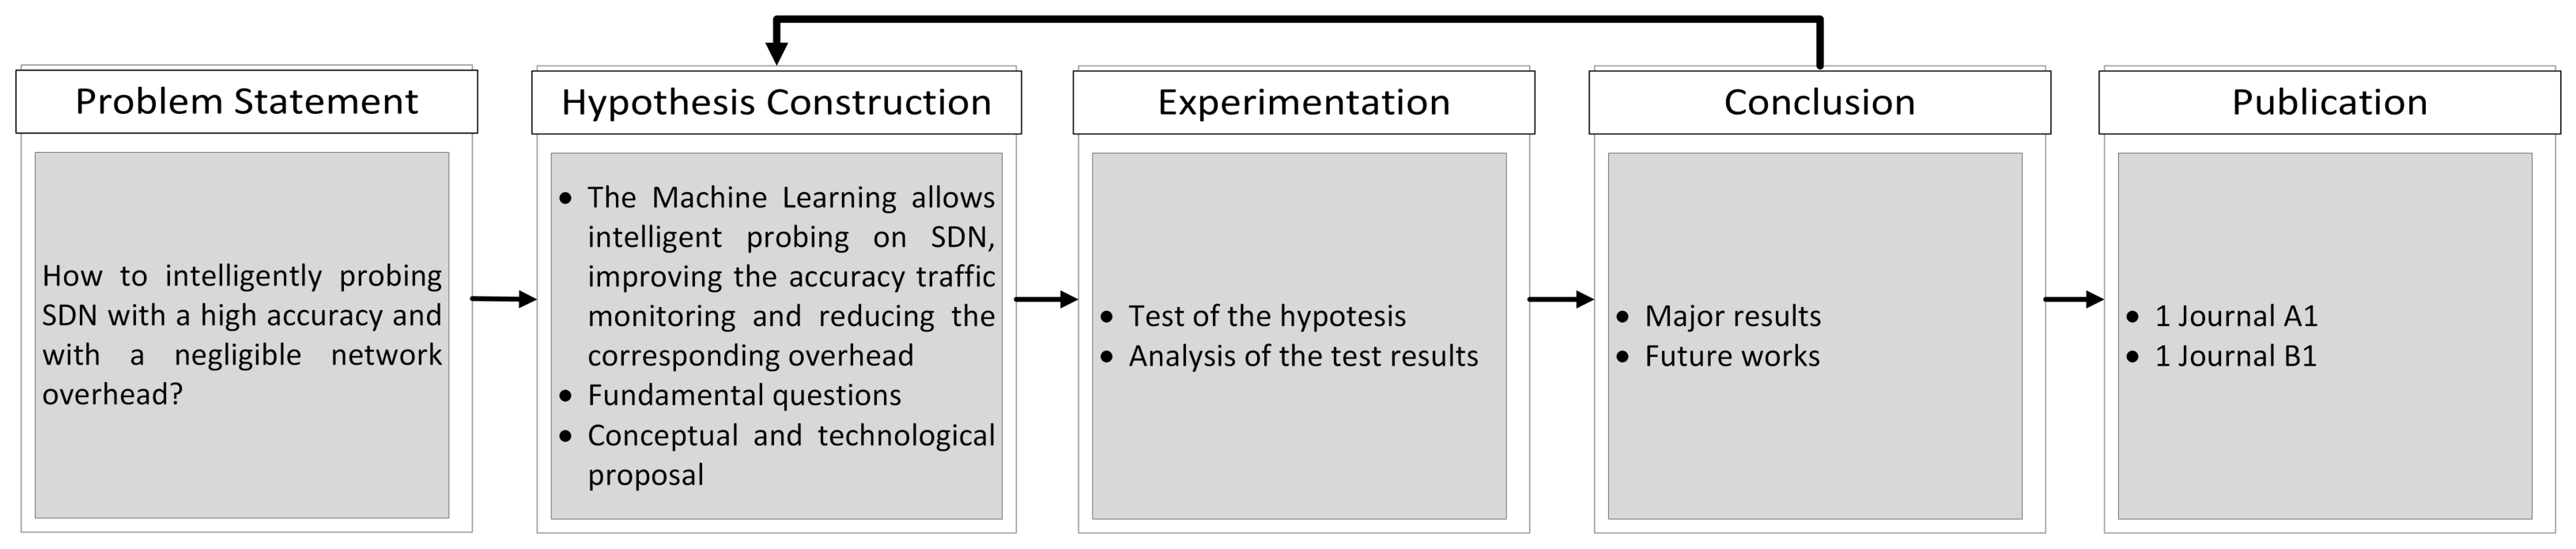
\includegraphics[width=1.0\columnwidth]{figures/scientific_research_process}
    \caption{Thesis phases}
    \label{fig:scientific_research_process}
\end{figure}

The organization of this document reflects the phases outlined above.
\begin{itemize}
    \item \textbf{This introductory chapter} presents the problem definition, raises the hypothesis, summarizes the contributions, and describes the overall structure of this master dissertation.
    
    \item \textbf{Chapter 2} reviews research about SDN, TE, Network Monitoring, ML, and KDN.
    
    \item \textbf{Chapter 3} presents the related works about SDN monitoring.
    
    \item \textbf{Chapter 4} presents a motivating scenario for the proposed approach. Also, this chapter introduces IPro, its architectural elements, and algorithmic representation.
    %introduces in detail the major contributions accomplished with this master dissertation.
    
    \item \textbf{Chapter 5} describes the experiments conducted to test the hypothesis, discusses the corresponding results, and presents implementation highlights.
    
    \item \textbf{Chapter 6} presents conclusions about the hypothesis and the fundamental questions, as well as opportunities for future works. 
    
    \item \textbf{Appendix} includes the list of papers in which the major results obtained during the development of this master dissertation have been published or submitted.
    
\end{itemize}